\documentclass[12pt,a4paper]{article}
\usepackage[utf8]{inputenc}
\usepackage{amsmath}
\usepackage{amsfonts}
\usepackage{amssymb}
\usepackage{graphicx}
\usepackage{polski}
\usepackage{mathtools}
\usepackage[utf8]{inputenc}
\DeclarePairedDelimiter{\ceil}{\lceil}{\rceil}

\title{Rozmieszczanie kamer bezpieczeństwa}
\author{Przemysław Kopański \\ Mateusz Forc}

\begin{document}
\maketitle
\tableofcontents
\section{Treść zadania}
Jak optymalnie rozmieścić kamery monitoringu w ustalonym pomieszczeniu (rzut z góry),
aby minimalną liczbą kamer móc obserwować dowolne miejsce 
(z uwzględnieniem maksymalnej dopuszczalnej odległości od kamery).
%
\newpage
\section{Przyjęte założenia}
\begin{itemize}
\item wszystkie kamery są takie same (mają taki sam zasięg)
	\begin{itemize}
	\item zasięg kamery jest kołem o stałym promieniu
	\item promień zasięgu kameru wynosi 2 (możliwa interpretacja - średnica kamery wynosi 4 metry)
	\end{itemize}
\item rzut pomieszczenia reprezentowany jest przez zbiór punktów
	\begin{itemize}
	\item punkty mają współrzędne odpowiadające I ćwiartce wykresu \[x \geq 0, y \geq 0\]
	\item punkty podawane są jako lista, która reprezentuje zamknięty wielokąt - muszą one zostać
	      podane we właściwej kolejności, tak aby można je było jednoznacznie połączyć 
	      (każde dwa kolejne punkty łączone są w odcinek)
	\end{itemize}
\end{itemize}
%
\section{Przestrzeń przeszukiwań}
Pojedynczym elementem przestrzeni przeszukiwań jest zbiór kamer wraz z ich pozycjami. \\
Rozwiązanie początkowe zawiera zbiór składający się z $\lceil$obszar rzutu/obszar jednej kamery$\rceil$ kamer
rozmieszczonych losowo wewnątrz wielokątu.
Do kolejnego stanu możemy przejść poprzez dodanie/usunięcie kamery lub przemieszczenie
jednej z aktualnie umieszczonych kamer.
Do zbioru kamer nie można wstawić kamery, która jest na zewnątrz obserwowanego pomieszczenia.
%
\newpage
\section{Funkcja celu}
Dostępna informacja: \\
\footnotesize
$k_{min}$ - minimalna teoretyczna liczba kamer dla aktualnie rozpatrywanego rzutu \\ \indent ($\lceil$obszar rzutu/obszar jednej kamery$\rceil$) \\
\normalsize
%
\newline
Parametry zadania: \\
$d_k$ - koszt użycia kamery \\
$d_p$ - wartość pokrycia 1\% powierzchni\\
\newline
Funkcja:
$f(p, k) = d_p*p - \frac{100d_k}{k_{min}}*max(k,k_{min}) $ \\ \\
gdzie: \\
p - \% pokrycia dla danego stanu \\
k - ilość użytych kamer w danym stanie \\ \\
Zadanie polega na maksymalizacji funkcji f. \\ \\ 
Przykładowo \\
$ d_p = 1 d_k = 1$ \\ \\ 
Dla podanych parametrów algorytm będzie znajdował ,,złoty środek pomiędzy'' 
procentem pokrycia a ilością użytych kamer.
Odpowiednio przeskalowując podane parametry i trzymajac odpowiedni 
stosunek pomiędzy tymi wartościami,
mozemy sterowac na czym bardziej nam zależy, jeżeli np 
$d_p = 2d_k = 1 $ to będziemy w stanie zaakceptować dwukrotna 
ilość kamer w zamian za dwukrotnie większe pokrycie.
%
\subsection{Przykład}
\begin{center}
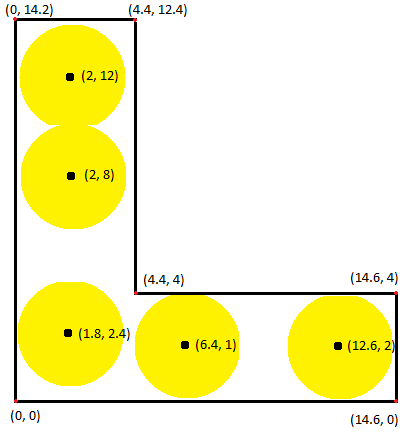
\includegraphics[scale=0.9]{example_projection.png}
\end{center}
Podane pomieszczenie ma pole powierzchni równe 103.38. \\
Zasięgi kamer są między sobą rozłączne, a ich pole wynosi 62.83. \\
Minimalna teoretyczna liczba kamery wynosi 9. \\
Pokrycie dla danego stanu wynosi 60.8\%. \\ \\
Dla parametrów:
$d_p = 1 d_k = 1$ \\
wartość funkcji wynosi 60.8-100 = -39.2 \\ \\
Podane rozwiązanie posiada zbyt małą liczbę kamer.
\section{Metaheurystyka}
Zastosowany zostanie stabuizowany algorytm symulowanego wyżarzania.
Ze względu na to, że stworzenie funkcji heurystycznej do badanej przestrzeni jest obliczalnie
trudne, użycie metody A* jest niewskazane.
Algorytmy wspinaczkowe nie sprawdzą się w opisywanej przestrzeni ze względu na dużą liczbę
ekstremów lokalnych. Stosując algorytm symulowanego wyżarzania zapewnione jest,
że algorytm nie ‘utknie’ w ekstremum. Wraz z rosnącą liczbą iteracji można zmniejszać temperaturę,
w celu znalezienia coraz lepszego rozwiązania. Dodatkowym mechanizmem pozwalającym uniknąć
zakotwiczenia w ekstremum lokalnym jest tabuizacja.\\

Podana metoda wymaga strojenia ze względu na 2 parametry:
\begin{enumerate}
  \item wielkość kolejki tabu - określa ile maksymalnie jednocześnie punktów przestrzeni może ulec tabuizacji
  \item parametr funkcji temperatury - do doboru temperatury zostanie wykorzystana funkcja zależna od numeru iteracji, która udostępni parametr do strojenia
\end{enumerate}
\section{Przewidywane wyniki pracy}
Dla kilkunastu zadanych rzutów ilustrujących różne warianty pomieszczeń np. długie, wąskie i kręte,
duże otwarte zostaną przeprowadzone symulacje w celu odnalezienia i zaprezentowania
parametrów funkcji celu, które pozwalają implementacji na znalezienie możliwie
najlepszego rozwiązania dla danego rodzaju przypadku. \\ \\
Wyniki zostaną zaprezentowane jako zestawy rzutów oraz wykresów
ilustrujących pokrycie w zależności od parametrów: $d_p$ i $d_k$ wraz z wyróżnionym zestawem
parametrów dla każdego zestawu, który ilustruje najlepsze rezultaty.
\end{document}
